	\documentclass{article}
\usepackage[colorlinks,citecolor=blue,urlcolor=blue]{hyperref}

\def\bbdot{\dot{\bb}}
\def\bgdot{\dot{\bg}}
\def\gdot{\dot{g}}
\def\ccdot{\dot{c}}
\def\adot{\dot{\ba}}
\def\bdot{\dot{\bb}}
\def\tdot{\dot{\bt}}
\def\tdd{\ddot{t}}
\def\addd{\ddot{a}}
\def\bdd{\ddot{b}}
\def\thetadot{\dot{\btheta}}
\def\covhat{\widehat{\cov}}
\def\siv{_{\text{IV}}}
\def\spp{_{\text{PP}}}
\def\sat{_{\text{AT}}}
\def\stsls{_{\text{TSLS}}}
\def\xpp{X\spp}



\usepackage[margin=1in]{geometry}
\usepackage{lmodern}
\usepackage{amsmath}               
\usepackage{graphicx}

\usepackage[T1]{fontenc}
\title{Synthetic compliance estimation}
\RequirePackage{amsthm,amsmath,geometry,amsfonts}
\RequirePackage{natbib}
\usepackage[utf8]{inputenc}
\usepackage[english]{babel}
\input{GrandMacros}
\input{Macro}

\newtheorem{assumption}{Assumption}
\begin{document}
\maketitle

\section{Introduction}

Compliance is an important issue in many experimental and observational studies. Patients who in experimental studies are randomized to receive treatment may not take it, and thus the typical intention-to-treat (ITT) analysis may not capture the effect of actually receiving treatment. Similarly, in observational data when a natural experiment occurs, those who gain access to a service or program may not take advantage of it. In these cases, reasons for non-compliance may be unavailable to researchers, and thus direct estimation of the effect of the intervention may not be possible because of unmeasured confounding. In these cases, researchers typically invoke assumptions, specify models, and possibly restrict the population of interest to identify the causal effect of the treatment. 

Many such choices of assumptions and models (and thus estimators) are available. Two simple examples are the as-treated (AT) estimator, where treatment is assumed to be essentially unconfounded after accounting for observed covariates, and the per-protocol (PP) estimator, where the analysis is restricted to those who followed their treatment assignment. Another set of estimators arises from the instrumental variables (IV) literature, where the assumption that treatment assignment is only related to the outcome through treatment receipt is leveraged. See \cite{imbens2014instrumental} for a detailed survey of methods and development in this space. Typically, researchers examine a range of (untestable) assumptions about the various estimators and select one. 

However, no one estimator will always outperform the others (see, e.g., \cite{Little2018, antonelli2017synthetic} for such a discussion of the estimators described above). Therefore, it is often beneficial to borrow information from all available estimators by creating a synthetic estimator as an optimal combination of all candidate estimators. This type of approach has received a lot of attention in the world of model averaging, where the coefficients from a series of (typically nested) regression models are considered as candidate estimators (see \cite{hjort2003frequentist, hansen2007least} as prominent examples). Comparatively less attention has been paid to averaging non-regression-based estimators or estimators of causal parameters. An exception is \cite{lavancier2016general}, who outline synthetic estimators for a very general class of problems and provide some asymptotic results. Another exception is \citet{antonelli2017synthetic}, who consider a synthetic estimator for the complier average causal effect (CACE) in the presence of non-compliance in the setting of a randomized controlled trial with no covariates measured. There they show that synthetic estimation can provide robustness in that, while the synthetic estimator is typically not better than all candidate estimators (as measured by MSE), it is typically competitive with the best estimators and much better than the worst ones. 

In the spirit of \citet{antonelli2017synthetic}, We propose a class of synthetic estimators (SCEs) which optimally combine candidate estimators of the CACE by minimizing the mean squared error (MSE) of the resulting estimator. The proposed estimators are appropriate for observational studies, and studies where covariates are to be included in the analysis.  The SCE displays a robustness property which allows it to take advantage of high-bias/low-variance estimators in situations where that is advantageous without sacrificing too  much performance when it is not. %We demonstrate that, under certain conditions, the SCE is asymptotically equivalent to the oracle estimator, the best possible synthetic estimator. 

The rest of the paper is organized as follows. In Section 2, we outline specifics about compliance and lay out the specific estimators we are considering in this work. In Section 3, we define the SCEs and deal with their practical implementation. Asymptotics are discussed in Section 4, and Section 5 includes simulations demonstrating the robustness of the approach. Section 6 contains concluding remarks.

\section{Compliance preliminaries}
Suppose the data for analysis consist of $n$ random vectors $(Y_i, Z_i, S_i, \bX_i)$ where $Y_i$ is the outcome, $Z_i$ is the treatment assignment, $S_i$ is an indicator of treatment, and $\bX_i$ is a set of covariates, all obtained on individual $i$. We assume throughout that treatment and compliance are binary, so that $Z_i, S_i$ take values in $\{0, 1\}$. Define the potential treatment indicators $S_i(0), S_i(1)$ to be the treatment status that would have been observed under the assignment of control ($Z_i = 0$) and treatment ($Z_i = 1$), respectively. Further define the principal strata to be defined by the random variable $\bU_i = \{S_i(0), S_i(1)\} \in \{0,1\}^2$. To map these principal strata to the framework used in \cite{Angrist1995} and \cite{Little2018}, {\em never-takers} have $\bU_i = (0, 0)$, {\em always-takers} have $\bU_i = (1, 1)$, {\em compliers} have $\bU_i = (0, 1)$, and {\em defiers} have $\bU_i = (1, 0)$. Define the potential outcomes $Y_i(0)$ and $Y_i(1)$ to be the outcomes that would have been observed under control and treatment, respectively, for patient $i$.  

Throughout, we make a series of assumptions that are standard in estimation with non-compliance and instrumental variables. First, we assume the Stable Unit Treatment Value Assumption (SUTVA) holds \cite{rubin1978bayesian} . That is, that the potential outcomes and potential treatment values for individual $i$ do not depend on any other individual. We further assume that $Z_i$ is a true instrument
\begin{align}
    \left.Z_i \amalg \left\{S_i(0), S_i(1), Y_i(0), Y_i(1)\right\}\right|\bX_i.
\end{align}
This ensures that the instrument is essentially randomly assigned within strata defined by $\bX_i$ and is similar to the no-unmeasured-confounders assumption commonly invoked for treatment effect estimation. Our third assumption requires that monotonicity holds, which means that there are no defiers and the treatment assignment does not make anyone less likely to receive the treatment. For simplicity, we will also assume so-called strong monotonicity
\begin{align}
    S_i(0) = 0. \label{strong_monotonicity}
\end{align}
This removes the possibility of always-takers from the population, as well, and simplifies our presentation here. Fourth, we assume the so-called exclusion restriction (ER)
\begin{align}
    E[Y_i(0) | \bU_i = (0, 0)] = E[Y_i(1) | \bU_i = (0, 0)]. \label{er}
\end{align}
which states that there is no direct effect of the treatment assignment on the outcome. If only monotonicity were assumed, then ER would mean that $E[Y_i(0) | \bU_i = (1, 1)] = E[Y_i(1) | \bU_i = (1, 1)]$, too. In some observational situtations, ER may be suspect, while in many randomized controlled trials in health it may be reasonable. It is finally typical to assume that the treatment assignment is related to whether someone takes the treatment. 

In addition to the above assumptions, we also consider one other assumption that is only needed for the AT and PP estimators. Specifically, this assumes that there exists no compliance effect among the controls conditional on $\bX_i$ (NCEC):
\begin{align}
    E[Y_i(0) | \bU_i = (0, 1), \bX_i] = E[Y_i(0) | \bU_i = (0, 0), \bX_i]. \label{ncec}
\end{align}
The NCEC assumption states that compliers and never-takers have similar outcomes under control. 


The target of estimation is the complier average causal effect (CACE) 
\begin{align}
\tau = E\{Y_i(1) - Y_i(0) | \bU_i = (0,1)\}. \label{cace}
\end{align}

%It is typical to assume that there are no defiers in the population, and in some situations where patients do not have independent access to the treatment, always-takers may be assumed away as well. Both are ensured by the so-called strong monotonicity assumption which can be found in \cite{Ding2017}:

%\begin{assumption}\label{strong_monotonicity}
%Strong monotinicity. \[
%S_i(0) = 0
%\]
%\end{assumption}

%Define the complier average causal effect (CACE) to be $$\tau = E\{Y_i(1) - Y_i(0) | \bU_i = (0,1)\}.$$ Define also the principle score to be $e(\bx) = P(\bU_i = (0,1) | \bX_i = \bx)$. Define similar but unconditional quantities $\pi_{11} = P(\bU_i = (1,1) | Z_i = 0)$ and $\pi_{00} = P(\bU_i = (0,0) | Z_i = 1)$. Let $n_0 = \sum_{i=1}^n I\{Z_i = 0\}$ and $n_1 = \sum_{i=1}^n I\{Z_i = 1\}$ be the treatment assignment sample sizes, and let $\ntilde_0 = \sum_{i=1}^n I\{S_i = 0\}$ and $\ntilde_1 = \sum_{i=1}^n I\{S_i = 1\}$ be the actual observed treatment sample sizes.

% \subsection{Assumptions}

% In this section we lay out various assumptions that may be used to justify various estimators of the CACE. These assumptions are adapted from \cite{Little2018} and \cite{Ding2017}. 

% \begin{assumption}[SUTVA]\label{sutva}
% Stable unit treatment value assumption.
% \end{assumption}

% \begin{assumption}\label{randomization}
% Randomization. 
% \[
% Z_i \amalg \left\{S_i(0), S_i(1), Y_i(1), Y_i(0), \bX_i\right\}
% \]
% \end{assumption}

% \begin{assumption}\label{monotonicity}
% Monotinicity. \[
% S_i(1) \geq S_i(0)
% \]
% \end{assumption}

% \begin{assumption}\label{strong_monotonicity}
% Strong monotinicity. \[
% S_i(0) = 0
% \]
% \end{assumption}

% \begin{assumption}[NCEC]\label{ncec}
% No compliance effect among the controls. %\[Y_i(0) \amalg \bU_i | U_{i1} = 0, Z_i = 0, \bX_i\]
% \[
% E[Y_i(0) | \bU_i = (0, 1)] = E[Y_i(0) | \bU_i = (0, 0)]
% \]
% \end{assumption}
% Note that Assumption \ref{ncec} is labeled NCEC$_\mu$ in \cite{Little2018}, while a stronger version is labeled NCEC:  $Y_i(0) \amalg \bU_i | U_{i1} = 0, Z_i = 0$. We stick with the weaker assumption on expectations here. 



% \begin{assumption}[Conditional NCEC v2]\label{cncec2}
% No compliance effect among the controls conditional on never-taker principal score $e\{(0,0); \bX_i\}$. %\[Y_i(0) \amalg \bU_i | U_{i1} = 0, Z_i = 0, \bX_i\]
% \[
% E[Y_i(0) | \bU_i = (0, 1), e\{(0,0); \bX_i\}] = E[Y_i(0) | \bU_i = (0, 0), e\{(0,0); \bX_i\}]
% \]
% \end{assumption}

% \begin{assumption}[NCET]\label{ncet}
% No compliance effect among the treated. %\[Y_i(1) \amalg \bU_i | U_{i2} = 1, Z_i = 1, \bX_i\]
% \[
% E[Y_i(1) | \bU_i = (0, 1)] = E[Y_i(1) | \bU_i = (1, 1)]
% \]
% \end{assumption}



% \begin{assumption}[ER]\label{er}
% Exclusion restriction. 
% \[
% %\left\{Y_i(0), Y_i(1)\right\} \amalg Z_i | \bU_i = (0, 0), \bX_i; \qquad
% %\left\{Y_i(0), Y_i(1)\right\} \amalg Z_i | \bU_i = (1, 1), \bX_i
% E[Y_i(0) | \bU_i = (0, 0)] = E[Y_i(1) | \bU_i = (0, 0)]; \qquad
% E[Y_i(0) | \bU_i = (1, 1)] = E[Y_i(1) | \bU_i = (1, 1)]
% \]
% \end{assumption}

% % \begin{assumption}[Conditional ER]\label{cer}
% % Exclusion restriction conditional on $\bX_i$. 
% % \[
% % %\left\{Y_i(0), Y_i(1)\right\} \amalg Z_i | \bU_i = (0, 0), \bX_i; \qquad
% % %\left\{Y_i(0), Y_i(1)\right\} \amalg Z_i | \bU_i = (1, 1), \bX_i
% % E[Y_i(0) | \bU_i = (0, 0), \bX_i] = E[Y_i(1) | \bU_i = (0, 0), \bX_i]; \qquad
% % E[Y_i(0) | \bU_i = (1, 1), \bX_i] = E[Y_i(1) | \bU_i = (1, 1), \bX_i]
% % \]
% % \end{assumption}

% \begin{assumption}[PI]\label{pi}
% Principal ignorability.
% \[
% Y_i(0) \amalg \bU_i | \bX_i
% \]
% \end{assumption}
% Note that this may(?) be a stronger assumption than the stronger version of Assumption \ref{ncec}. 

% \begin{assumption}[GPI]\label{gpi}
% Generalized principal ignorability.
% \[
% Y_i(0) \amalg \bU_i | \bX_i; \qquad Y_i(1) \amalg \bU_i | \bX_i
% \]
% \end{assumption}

% % \begin{assumption}
% % Stratification sufficiency. 

% % \end{assumption}


\subsection{Candidate CACE estimators}
For clarity and ease of presentation, we restrict ourselves to a series of well-known estimators for the CACE. The SCE could easily be adapted to include other candidate estimators with ease. 

Let $\Shat(\bX_i)$ be an estimate of $E[S_i | \bX_i]$, which is typically obtained froma linear regression of $S_i$ on $\bX_i$. Let $X$ be the the design matrix with $i$th row $\bX_i$, and let $X_\Shat$ be $X$ augmented with the column $\bShat = (\Shat_1, ..., \Shat_n)$. Let $\bY = (Y_1, .., Y_n)$ and $\bS = (S_1, .., S_n)$. Define $\xpp$ to be a submatrix of $X$ such that it only includes rows where $S_i = Z_i$: $\xpp = (X_i)_{S_i = Z_i}$. Similarly, define $S\spp = (S_i : S_i = Z_i), Y_\spp = (Y_i : S_i = Z_i)$. Further, define $\pi_{00} = P(\bU_i = (0,0) | Z_i = 1)$, and let $n_0 = \sum_{i=1}^n I\{Z_i = 0\}$ and $n_1 = \sum_{i=1}^n I\{Z_i = 1\}$ be the treatment assignment sample sizes.

We consider the following four estimators
\begin{align}
    &\tauhat\siv = \frac{n_1\inv\sum_{i=1}^nY_iI\{Z_i = 1\} - n_0\inv\sum_{i=1}^nY_iI\{Z_i = 0\}}{1 - \pihat_{00}} \label{iv_est} \\
    &\tauhat\stsls = (X_\Shat\trans X_\Shat)\inv \bShat\trans \bY  \label{tsls_est}\\
    &\tauhat\sat = (X\trans X)\inv \bS\trans \bY \label{at_est}\\
    &\tauhat\spp = (\xpp\trans\xpp)\inv \bS\spp\trans \bY\spp\label{pp_est}
\end{align}
These estimators correspond to the typical IV estimator, $\tauhat\siv$, the typical two-stage least-squares estimator, $\tauhat\stsls$, the as-treated (AT) estimator $\tauhat\sat$, and the per-protocol (PP) estimator, $\tahat_spp$. See \cite{Little2018} for a discussion of the IV, AT, and PP estimators, and see \cite{antonelli2017synthetic} for a comparison of these estimators in the situation without covariates. 

% \paragraph{Vanilla IV.} Under Assumptions \ref{strong_monotonicity}, \ref{sutva}, and \ref{er}, the following estimator is consistent for the CACE \[
% \tauhat\siv(0, 1) = \frac{n_1\inv\sum_{i=1}^nY_iI\{Z_i = 1\} - n_0\inv\sum_{i=1}^nY_iI\{Z_i = 0\}}{1 - \pihat_{00}}
% \]
% provided that $\pi_{00}$ is estimated consistently. The exclusion restriction guarantees that the instrument has no effect on the mean counterfactual outcome in the never-takers. 

% In a similar vein, we can propose a model-based two-stage least squares estimator, where we first regress $S_i$ onto $\bX_i$ in the treated group (does this require strong monotonicity?). Then, we obtain a prediction for $S_i(\bX_i)$ among all subjects, which we call $\Shat(\bX_i)$, and then regress $Y_i$ onto $\Shat(\bX_i)$ and $\bX_i$.

% \paragraph{Two-stage least squares.} Under Assumptions \ref{strong_monotonicity}, \ref{sutva}, and \ref{er}, the coefficient corresponding to $\Shat(\bX_i)$ in a regression of $Y_i$ onto $\Shat(\bX_i)$ and $\bX_i$ will be consistent for the CACE as long as $\Shat(\bX_i) \rightarrow P(S_i = 1 | \bX_i)$ and the regression model is correctly specified.  

% We also consider two other assumptions and estimators. 

% \begin{assumption}[Conditional NCET]\label{cncet1}
% No compliance effect among the treated conditional on $\bX_i$. 
% \[
% E[Y_i(1) | \bU_i = (0, 1), \bX_i] = E[Y_i(1) | \bU_i = (1, 1), \bX_i]
% \]
% \end{assumption}

% \begin{assumption}[Conditional NCEC]\label{cncec1}
% No compliance effect among the controls conditional on $\bX_i$. %\[Y_i(0) \amalg \bU_i | U_{i1} = 0, Z_i = 0, \bX_i\]
% \[
% E[Y_i(0) | \bU_i = (0, 1), \bX_i] = E[Y_i(0) | \bU_i = (0, 0), \bX_i]
% \]
% \end{assumption}

% These assumptions give rise to the per-protocol estimator:
% \paragraph{Conditional per-protocol.} Under Assumptions \ref{sutva}, \ref{cncec1} and \ref{cncet1}, the coefficient corresponding to $S_i$ from a regression of $Y_i$ on $S_i$ and $\bX_i$ among patients for whom $S_i = Z_i$ will be consistent for the CACE as long as the regression model is correctly specified. 

% A final estimator invokes both the exclusion restriction and NCEC/NCET:
% \paragraph{Conditional as-treated.} Under Assumptions \ref{sutva}, \ref{cncec1}, \ref{cncet1}, and \ref{er} the coefficient corresponding to $S_i$ from a regression of $Y_i$ on $S_i$ and $\bX_i$ will be consistent for the CACE as long as the regression model is correctly specified. 

\section{Synthetic estimation}

In this section, we propose a series of synthetic estimators which leverage the information in all candidate estimators. Let the set of candidate estimators be $\bthetahat = (\thetahat_0, \thetahat_1, ..., \thetahat_k) = (\thetahat_0, \bthetahat_1)$, where $\thetahat_0$ is an estimator that can be presumed to be unbiased, and $\bthetahat_1$ collects all other candidates. Define $\cov(\bthetahat) = \Sigma$ and $E[\bthetahat - \theta] = \bDelta = (0, \Delta_1, ..., \Delta_k)$. Because the exclusion restriction (\ref{er}) can often be plausibly assumed to hold, we typically consider either the vanilla IV estimator or the TSLS estimator to be $\thetahat_0$: either $\bthetahat = (\tauhat\siv, \tauhat\stsls, \tauhat\sat, \tauhat\spp)$ or $\bthetahat = (\tauhat\stsls, \tauhat\siv, \tauhat\sat, \tauhat\spp)$. When the assumption (\ref{er}) is deemed unlikely, another estimator may be considered as $\thetahat_0$. 

We consider a synthetic estimator as a convex combination of the candidates \[
\theta_s(\bb) = \bb\trans\bthetahat = b_0\thetahat_0 + \bb_1\trans\bthetahat_1
\]
where $\bb \in \Bsc = \left\{\ba = (a_1, ... a_{k+1}): \bone_{k+1}\trans\ba = 1, a_i \geq 0\right\}$, so that $\bone_k\trans\bb_1 = 1 - b_0$. The synthetic estimator aims to improve on the unbiased $\theta_0$ by lowering its overall mean squared error (MSE) by including the (possibly biased) $\bthetahat$ in the hopes of attaining lower variance.

To balance bias and variance, the linear combination $\bbtilde$ would ideally be chosen to directly minimize the MSE:
\begin{align}
    \bb^* = \argmin{\bb}MSE(\theta_s(\bb))
\end{align}
where 
\begin{align*}
\text{MSE}(\thetahat_s) &= E[(\thetahat_s - \btheta)^2] = E[(\bb\trans\bthetahat - \btheta)^2]\\
%&= \bbtilde\trans\cov(\bthetatilde)\bbtilde + (\bbtilde\trans E[\bthetatilde] - \theta)^2\\
%&= \bbtilde\trans\cov(\bthetatilde)\bbtilde + (\bb\trans E[\btheta] - \theta)^2\\
&= \bb\trans\Sigma\bb + (\bb\trans \bDelta)^2.
\end{align*}

Of course, $\Sigma$ and $\bDelta$ are unknown a priori. The proposed estimator is then a plug-in estimator, based on estimates of $\Sigma$ and $\bDelta$,
\begin{align}
    \thetahat_s = \theta_s(\bbhat) = \bhat_0\thetahat_0 + \bbhat_1\trans\bthetahat_1
\end{align}
where $ \bbhat = \argmin{\bb}\widehat{MSE}(\theta_s(\bb)) = \argmin{\bb}\bb\trans\Sigmahat\bb + (\bb\trans \bDeltahat)^2$. 

It is typically straightforward to compute $\Sigmahat$ by using for example the bootstrap. On the other hand, when it comes to estimating $\bDeltahat$, the situation is much more difficult. If we, for example, knew $\bDeltahat$, which corresponds to the bias in each candidate estimator, then we could just correct the bias in the candidate with the lowest variance. Despite this difficulty, we propose in the following some useful plug-in $\bDeltahat$s.

\paragraph{Bias estimate: raw differences.}
Because we assume that $\bthetahat_0$ is unbiased, we can estimate the bias in the other estimators by taking their raw differences with $\bthetahat_0$:
\[
\bDeltahat_r = (0, \thetahat_1 - \thetahat_0, ..., \thetahat_k - \thetahat_0).
\]
This results in the estimator $\thetahat_{sr} = \theta_s(\bbhat_r)$ where $\bbhat_r = \argmin{\bb}\bb\trans\Sigmahat\bb + (\bb\trans \bDeltahat_r)^2$.

\paragraph{Bias estimate: modified raw differences.}
We know that the raw differences are not typically an accurate estimate of the bias, and they may tend to be highly variable. To ameliorate their variability, we may want to regularize the bias estimates by down-weighting the most highly variable ones: 
\[
\bDeltahat_m = \bw \cdot \bDeltahat_r
\]
where $\ba \cdot \bb = (a_1b_1, ..., a_kb_k)$ and $\bw = (w_0, ..., w_k)$ with
\[
w_j = \frac{\Deltahat_j^2}{\sigmahat_0 + \sigmahat_j - 2\sigmahat_{0j} + \Deltahat_j^2}
\]
and $\Sigmahat_{mn} = \sigma_{(m-1)(n-1)}$
If the bias $\Deltahat_j$ is large relative to $\widehat{\var}(\thetahat_1 - \thetahat_0)$, then the weight will be close to 1, meaning the bias is not shrunk very much. On the other hand, if the bias is small compared to the variance, the weight $w_j$ will be close to 0 and the bias will be shrunk toward 0. This results in the estimator $\thetahat_{sm} = \theta_s(\bbhat_m)$ where $\bbhat_m = \argmin{\bb}\bb\trans\Sigmahat\bb + (\bb\trans \bDeltahat_m0)^2$.
\paragraph{Sample-splitting approach.}
We also consider an approach which estimates the bias on an independent set of data. Consider splitting the available data into two equally sized datasets, and estimating the candidate estimators on each. Let $\bthetahat_a = (\thetahat_{a0}, ..., \thetahat_{bk}$ be the set of candidates estimated on one half, and $\bthetahat_b = (\thetahat_{b0}, ..., \thetahat_{bk}$ be estimated on the other half. And let $\bDeltahat_a = (0, \thetahat_{a1} - \thetahat_{a0}, ..., \thetahat_{ak} - \thetahat_{a0})$, and let $\bDeltahat_b$ be defined accordingly. 

We can then compute two sets of coefficients $\bbhat_a = \argmin{\bb}\bb\trans\Sigmahat\bb + (\bb\trans \bDeltahat_a)^2$ and $\bbhat_b = \argmin{\bb}\bb\trans\Sigmahat\bb + (\bb\trans \bDeltahat_b)^2$. We can then apply the coefficients computed on one half to the candidates from the other half and average the two:
\[
\thetahat_{ss} = \frac{1}{2}\bbhat_a\trans\bthetahat_b + \frac{1}{2}\bbhat_b\trans\bthetahat_a.
\]

\section{Asymptotic behavior}
In this section, we will discuss under what conditions the proposed estimators perform asymptotically as well as the optimal estimator. We subscript relevant estimators by $n$ here to make clear when quantities may change with $n$. Let $\Omega_n = \Sigma_n + \bDelta_n\bDelta_n\trans$, $\Omegahat_n = \Sigmahat_n + \bDeltahat_n\bDeltahat_n\trans$, and $\bS = \Omega_n\inv(\bthetahat - \theta)$. Then, according to Theorem 3.1 in \cite{lavancier2016general}, we obtain the finite-sample result
\begin{align*}
    (\thetahat_s - \theta^*)^2 \leq \deltatilde(\Omegahat_n, \Omega_n) \|\bS\|^2 E[(\theta^* - \theta)^2],
\end{align*}
where $\thetastar = \bbstar\trans\thetahat$, $\deltatilde(\Omegahat_n, \Omega_n) = 2\delta(\Omegahat_n, \Omega_n) + \delta(\Omegahat_n, \Omega_n)^2$ and $\delta(\Omegahat_n, \Omega_n) = \sup_{\bb \in \Bsc}\left|1 - \frac{\tr(\bb\trans\Omegahat_n\bb)}{\tr(\bb\trans\Omega_n\bb)}\right|$. This result limits the deviation of the synthetic estimator from the best possible synthetic estimator in terms of three terms: the error of the MSE estimator $\Omegahat_n$; the errzor of $\bthetahat$; and the MSE of the best possible synthetic estimator.

Under the assumption $\bthetahat = O_p(1)$ and thus $\bS = O_p(1)$, it is for $\Omegahat_n\Omega_n\inv \rightarrow I$ as $n \rightarrow \infty$ to ensure that 
\begin{align}
    (\thetahat_s - \theta^*)^2 = o_p(1).
\end{align}
Further, assuming $\pihat_{00} - \pi_{00} = O_p(\nnhalf)$ and $\bShat_n - \bStilde = O_p(\nnhalf)$, for $\lim_n \bShat_n$, $\Sigma_n = O_p(n\inv)$, and all standard estimators will converge at a similar rate $\Sigmahat_n = O_p(n\inv)$. Further, as long as $E[\thetahat_0] = 0$, $\bDeltahat - \bDelta = O_p(\nnhalf)$. 

\def\ddp{\bDelta_n\bDelta_n\trans}
\def\ddhp{\bDeltahat_n\bDeltahat_n\trans}
\def\dsd{\bDelta_n\trans\Sigma_n\inv\bDelta_n}
\begin{align*}
    (\Sigmahat_n + \ddhp)(\Sigma_n + \ddp)\inv &= \left(\Sigmahat_n\Sigma_n\inv + \ddhp\Sigma_n\inv\right)\left(I - \frac{ \ddp\Sigma_n\inv}{1 +\dsd}\right)\\
    &= \Sigmahat_n\Sigma_n\inv +\ddhp\Sigma_n\inv - \Sigmahat_n\Sigma_n\inv\frac{ \ddp\Sigma_n\inv}{1 +\dsd} - \ddhp\Sigma_n\inv\frac{ \ddp\Sigma_n\inv}{1 +\dsd}
\end{align*}

% \begin{assumption}[Conditional NCET]\label{cncet2}
% No compliance effect among the treated conditional on always-taker principal score $e\{(1,1); \bX_i\}$. %\[Y_i(1) \amalg \bU_i | U_{i2} = 1, Z_i = 1, \bX_i\]
% \[
% E[Y_i(1) | \bU_i = (0, 1), e\{\bX_i\}] = E[Y_i(1) | \bU_i = (1, 1), e\{\bX_i\}]
% \]
% \end{assumption}

% \paragraph{Per-protocol.} Under Assumptions \ref{sutva}, \ref{ncec} and \ref{ncet}, the following estimator is consistent for the CACE
% \[
% \tauhat\spp(0, 1) = \frac{\sum_{i=1}^nY_iI\{Z_i = 1, S_i = 1\}}{\sum_{i=1}^nI\{Z_i = 1,S_i=1\}} - \frac{\sum_{i=1}^nY_iI\{Z_i = 0, S_i = 0\}}{\sum_{i=1}^nI\{Z_i = 0,S_i=0\}}
% \]

% \paragraph{As-treated.} Under Assumptions \ref{sutva}, \ref{er}, \ref{ncec} and \ref{ncet}, the following estimator is consistent for the CACE
% \[
% \tauhat\sat(0, 1) = \ntilde_1\inv\sum_{i=1}^nY_iI\{S_i = 1\} - \ntilde_0\inv\sum_{i=1}^nY_iI\{S_i = 0\}
% \]

% %\cite{Little2018} took $\pihat_{11} = n_0\inv\sum_{i=1}^n I\{Z_i = 0, S_i = 1\}$ and $\pihat_{00} = n_1\inv\sum_{i=1}^n I\{Z_i = 1, S_i = 0\}$ to be the estimated proportion of always-takers and never-takers where $n_0 = \sum_{i=1}^n I\{Z_i = 0\}$ and $n_1 = \sum_{i=1}^n I\{Z_i = 1\}$. However, this doesn't seem right to me, as the $\pihat_{00}$ and $\pihat_{11}$ could easily sum to more than 1, ***right***?

% \paragraph{Conditional IV.} Under Assumptions \ref{sutva} and \ref{er}, the following estimator is consistent for the CACE
% \[
% \tauhat_{IVw}(0,1) = \frac{\sum_{i=1}^n\Deltahat_i}{\sum_{i=1}^n \ehat\{(0,1); \bX_i\}}
% \]
% provided $\Deltahat_i \longrightarrow E[Y_i(1) - Y_i(0) | \bX_i]$ and $\ehat\{(0,1); \bX_i\} \longrightarrow e\{(0,1); \bX_i\}$. **There's probably a weaker assumption to be made here**.

% \paragraph{Two-stage least squares.} Under Assumptions \ref{sutva} and \ref{er}, the coefficient corresponding to $\Shat(\bX_i)$ in a regression of $Y_i$ onto $\Shat(\bX_i)$ and $\bX_i$ will be consistent for the CACE as long as $\Shat(\bX_i) \rightarrow P(S_i = 1 | \bX_i)$ and the regression model is correctly specified.  

% \paragraph{Conditional per-protocol.} Under Assumptions \ref{sutva}, \ref{cncec2} and \ref{cncet2}, the coefficient corresponding to $S_i$ from a regression of $Y_i$ on $S_i$, $e\{(1,1); \bX_i\}$, $e\{(0,0); \bX_i\}$ among patients for whom $S_i = Z_i$ will be consistent for the CACE as long as the regression model is correctly specified. Alternatively, if $\bX_i$ is low-dimensional, under Assumptions \ref{sutva}, \ref{cncec1} and \ref{cncet1}, the coefficient corresponding to $S_i$ from a regression of $Y_i$ on $S_i$ and $\bX_i$ among patients for whom $S_i = Z_i$ will be consistent for the CACE as long as the regression model is correctly specified. 

% \paragraph{Conditional as-treated.} Under Assumptions \ref{sutva}, \ref{er}, \ref{cncec2} and \ref{cncet2}, the coefficient corresponding to $S_i$ from a regression of $Y_i$ on $S_i$, $e\{(1,1); \bX_i\}$, $e\{(0,0); \bX_i\}$ will be consistent for the CACE as long as the regression model is correctly specified. Alternatively, if $\bX_i$ is low-dimensional, under Assumptions \ref{sutva}, \ref{cncec1} and \ref{cncet1}, the coefficient corresponding to $S_i$ from a regression of $Y_i$ on $S_i$ and $\bX_i$ will be consistent for the CACE as long as the regression model is correctly specified. 

% \paragraph{Inverse-probability weighted (no never-takers).} Under Assumptions \ref{strong_monotonicity} and \ref{pi}, the following estimator is consistent for the CACE
% \[
% \tauhat_{IPW}(0, 1) = \frac{\sum_{i=1}^nY_iI\{Z_i = 1, S_i = 1\}}{{\sum_{i=1}^nI\{Z_i = 1,S_i=1\}}} - n_0\inv\sum_{i=1}^n\what_iY_iI\{Z_i = 0\}
% \]
% where $\what_i = \frac{\Phat(S_i = 1 | Z_i = 1, \bX_i)}{\Phat(S_i = 1 | Z_i = 1)} = \frac{\ehat\{(0,1); \bX_i\}}{\Phat(S_i = 1 | Z_i = 1)}$. 

% \paragraph{Inverse-probability weighted (general).} Under Assumptions \ref{strong_monotonicity} and \ref{pi}, the following estimator is consistent for the CACE
% \[
% \tauhat_{IPW}(0,1) = \frac{\sum_{i=1}^n w_1(\bX_i) Y_iI\{Z_i = 1, S_i = 1\}}{\sum_{i=1}^nI\{Z_i = 1,S_i=1\}} - \frac{\sum_{i=1}^n w_0(\bX_i) Y_iI\{Z_i = 0, S_i = 0\}}{\sum_{i=1}^nI\{Z_i = 0,S_i=0\}}
% \]
% where 
% \[
% w_1(\bX_i) = \frac{e\{(0,1); \bX_i\}}{e\{(0,1); \bX_i\} + e\{(1,1); \bX_i\}}(1-\pi_{11})\inv
% \]
% and \[
% w_0(\bX_i) = \frac{e\{(0,1); \bX_i\}}{e\{(0,1); \bX_i\} + e\{(0,0); \bX_i\}}(1-\pi_{00})\inv.
% \]


% $$
% \tauhat_{IPW}(0,1) = \frac{\sum_{i=1}^n w_1(\bX_i) Y_iI\{Z_i = 1, S_i = 1\}}{\sum_{i=1}^nI\{Z_i = 1,S_i=1\}} - \frac{\sum_{i=1}^n w_0(\bX_i) Y_iI\{Z_i = 0, S_i = 0\}}{\sum_{i=1}^nI\{Z_i = 0,S_i=0\}}
% $$
% where 
% $$
% w_1(\bX_i) = \frac{e\{(0,1); \bX_i\}}{e\{(0,1); \bX_i\} + e\{(1,1); \bX_i\}}(1-\pi_{11})\inv\\
% w_0(\bX_i) = \frac{e\{(0,1); \bX_i\}}{e\{(0,1); \bX_i\} + e\{(0,0); \bX_i\}}(1-\pi_{00})\inv.
% $$

% Define further the principle score to be $e(\bu; \bx) = P(\bU_i = \bu | \bX_i = \bx)$. We can then consider two stratified versions of the preceding estimators. First, define $K$ strata of $e\{(0,1); \bx\}$: $W_i = \sum_{k=1}^K I\left\{e\{(0,1); \bx\} \leq \ell_k\right\}, \ell_k \in [0,1]$. Take $\pihat_{11k} = n_{0k}\inv\sum_{i=1}^n I\{Z_i = 0, S_i = 1, W_i = k\}$ and $\pihat_{00k} = n_{1k}\inv\sum_{i=1}^n I\{Z_i = 1, S_i = 0, W_i = k\}$ to be the estimated proportion of always-takers and never-takers in the $k$th strata where $n_{0k} = \sum_{i=1}^n I\{Z_i = 0, W_i = k\}$ and $n_{1k} = \sum_{i=1}^n I\{Z_i = 1, W_i = k\}$. Let $\ntilde_{0k} = \sum_{i=1}^n I\{S_i = 0, W_i = k\}$ and $\ntilde_{1k} = \sum_{i=1}^n I\{S_i = 1, W_i = k\}$.

% The stratified estimators can then be estimated as
% $$
% \tauhat_{IVs}(0,1) = n\inv\sum_{k=1}^Kn_k\tauhat_{IVk}(0,1)\\
% \tauhat_{ATs}(0,1) = n\inv\sum_{k=1}^Kn_k\tauhat_{ATk}(0,1)\\
% \tauhat_{PPs}(0,1) = n\inv\sum_{k=1}^Kn_k\tauhat_{PPk}(0,1)
% $$
% where $n_k = \sum_{i=1}^n I\{W_i = k\}$ and

% $$
% \tauhat_{IVk}(0, 1) = \frac{n_{1k}\inv\sum_{i=1}^nY_iI\{Z_i = 1, W_i = k\} - n_{0k}\inv\sum_{i=1}^nY_iI\{Z_i = 0, W_i = k\}}{1 - \pihat_{00k} - \pihat_{11k}}\\
% \tauhat_{ATk}(0, 1) = \ntilde_{1k}\inv\sum_{i=1}^nY_iI\{S_i = 1, W_i = k\} - \ntilde_{0k}\inv\sum_{i=1}^nY_iI\{S_i = 0, W_i = k\}\\
% \tauhat_{PPk}(0, 1) = \frac{\sum_{i=1}^nY_iI\{Z_i = 1, S_i = 1, W_i = k\}}{\sum_{i=1}^nI\{Z_i = 1,S_i=1, W_i = k\}} - \frac{\sum_{i=1}^nY_iI\{Z_i = 0, S_i = 0, W_i = k\}}{\sum_{i=1}^nI\{Z_i = 0,S_i=0, W_i = k\}}
% $$

% In an identical fashion, we can follow Little's suggestion to create $K$ strata based on both $e\{(0,0); \bX\}$ and $e\{(1,1); \bX\}$. We can additionally follow Little's suggestion to use the following estimator
% $$
% \tauhat_{IVw}(0,1) = \frac{\sum_{i=1}^n\Deltahat_i}{\sum_{i1=1}^n \ehat\{(0,1); \bX_i\}}
% $$
% where $\Deltahat_{1i}$ is the predicted causal effect for indidividual $i$ based on some outcome model, which can be computed using a generalized random forest. *** What is the right denominator?***



% We can also consider regression versions of all the proposed estimators. Two-stage least-squares estimators for IV, where we first regress $S_i$ onto $\bX_i$ in the treated group (this is what Little suggests doing), and then regress $Y_i$ onto $\Shat(\bX_i)$ and $\bX_i$. For AT and PP, we can just regress $Y_i$ onto $S_i$ controlling for $\bX_i$ in all patients (for AT) or just among those who comply (for PP).



% We can finally use weighting estimators of the form
% $$
% \tauhat_{IPW}(0,1) = \frac{\sum_{i=1}^n w_1(\bX_i) Y_iI\{Z_i = 1, S_i = 1\}}{\sum_{i=1}^nI\{Z_i = 1,S_i=1\}} - \frac{\sum_{i=1}^n w_0(\bX_i) Y_iI\{Z_i = 0, S_i = 0\}}{\sum_{i=1}^nI\{Z_i = 0,S_i=0\}}
% $$
% where 
% $$
% w_1(\bX_i) = \frac{e\{(0,1); \bX_i\}}{e\{(0,1); \bX_i\} + e\{(1,1); \bX_i\}}(1-\pi_{11})\inv\\
% w_0(\bX_i) = \frac{e\{(0,1); \bX_i\}}{e\{(0,1); \bX_i\} + e\{(0,0); \bX_i\}}(1-\pi_{00})\inv.
% $$

\section{Simulation}
We adapt the simulation set-up in \cite{stuart2015assessing} which allows us to examine a range of assumptions. The model has the following form:
\begin{align}
Y_i = \alpha_c C_i + \gamma_cC_iZ_i + \lambda_n X_i + (\lambda_c - \lambda_n)C_iX_i + \epsilon_i
\end{align}
where $C_i = I\{\bU_i = (0, 1)\}$ is an indicator of being a complier. The CACE is identified by the parameter $\gamma_c$. And the model for compliance takes the form
\begin{align}
\logit(\pi_i) = \beta_0 + \beta_1X_i
\end{align}
where $P(C_i = 1 | X_i) = \pi_i$. %We assume strong monotocity (Assumption \ref{strong_monotonicity}) throughout. 
This model assumes the exclusion restriction (Assumption \ref{er}) holds.

Assumption \ref{cncec1} (NCEC)  can be ensured by setting \[
\alpha_c = 0 \text{ and } \lambda_n = \lambda_c.
\] 
Similarly, Assumption \ref{cncet1} (NCET) is ensured by 
\[
\alpha_c = 0, \gamma_c = 0, \text{ and } \lambda_n = \lambda_c.
\] 
We generated data at three sample sizes, $n = 200, 500, 1000$, and we varied the level of violation of Assumptions \ref{cncec1} and \ref{cncet1} by letting $\alpha_c$ take values in (0, 0.1, 0.2, 0.3, 0.4, 0.5).  We also allow $\lambda_n, \lambda_c$, and $\gamma_c$ to be 0 or 1. We considered the four candidate estimators, as well as synthetic estimators based on the Vanilla IV estimator and the TSLS estimator, respectively. 

The simulations demonstrate that the synthetic estimator has a robustness property. Consider Figure \ref{mse_plot_1}, which depicts one set of simulation results where $\alpha_c$ varies the degree to which the NCEC/NCET assumptions are violated. When $\alpha_c$ = 0, the NCEC/NCET assumptions hold, and the AT and PP estimators are unbiased. When $\alpha_c = 0.5$, the NCEC/NCET assumptions do not hold, and the AT and PP estimators incur bias. 
%
\begin{figure}
\centering
\begin{tabular}{c}
%\includegraphics{figure_1_correlations.eps}
%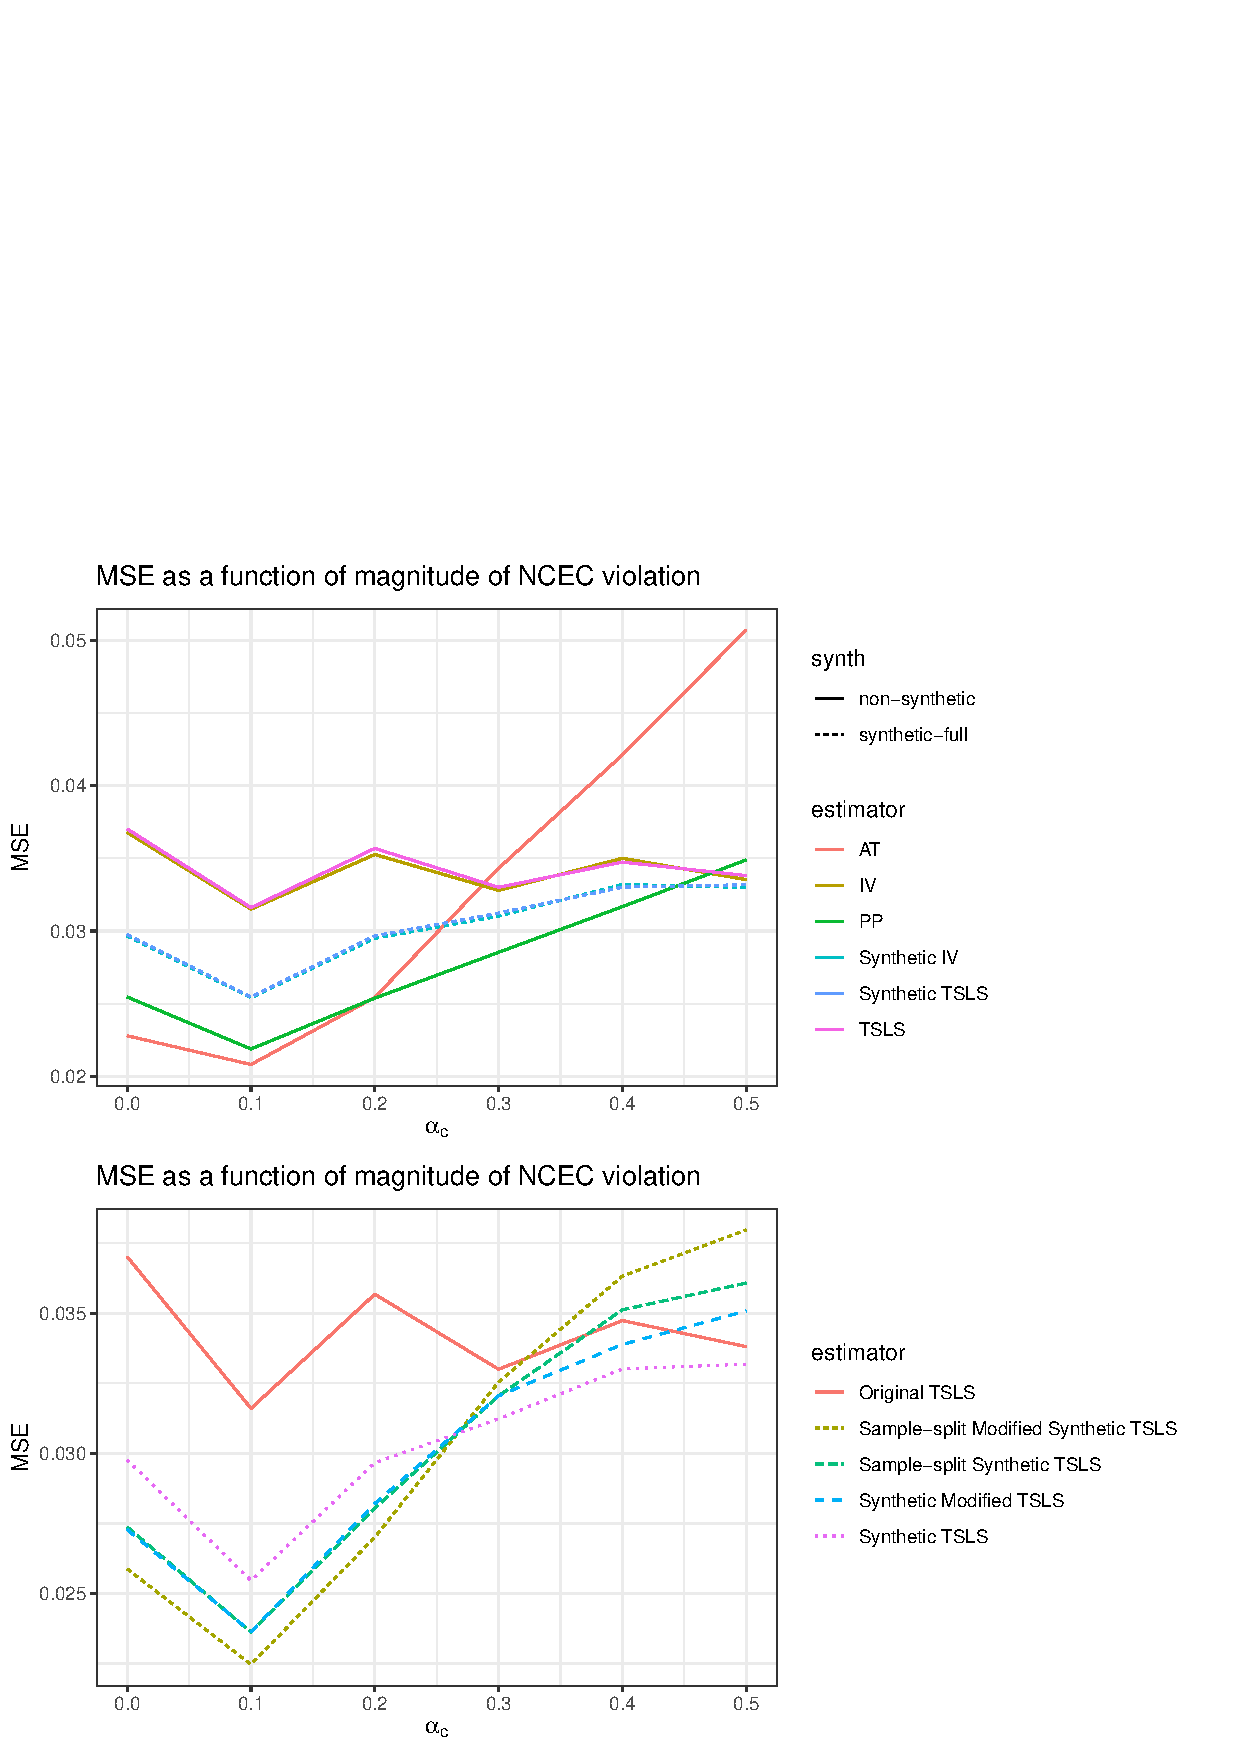
\includegraphics{mse_bias_var_for_n200_cp06.png}
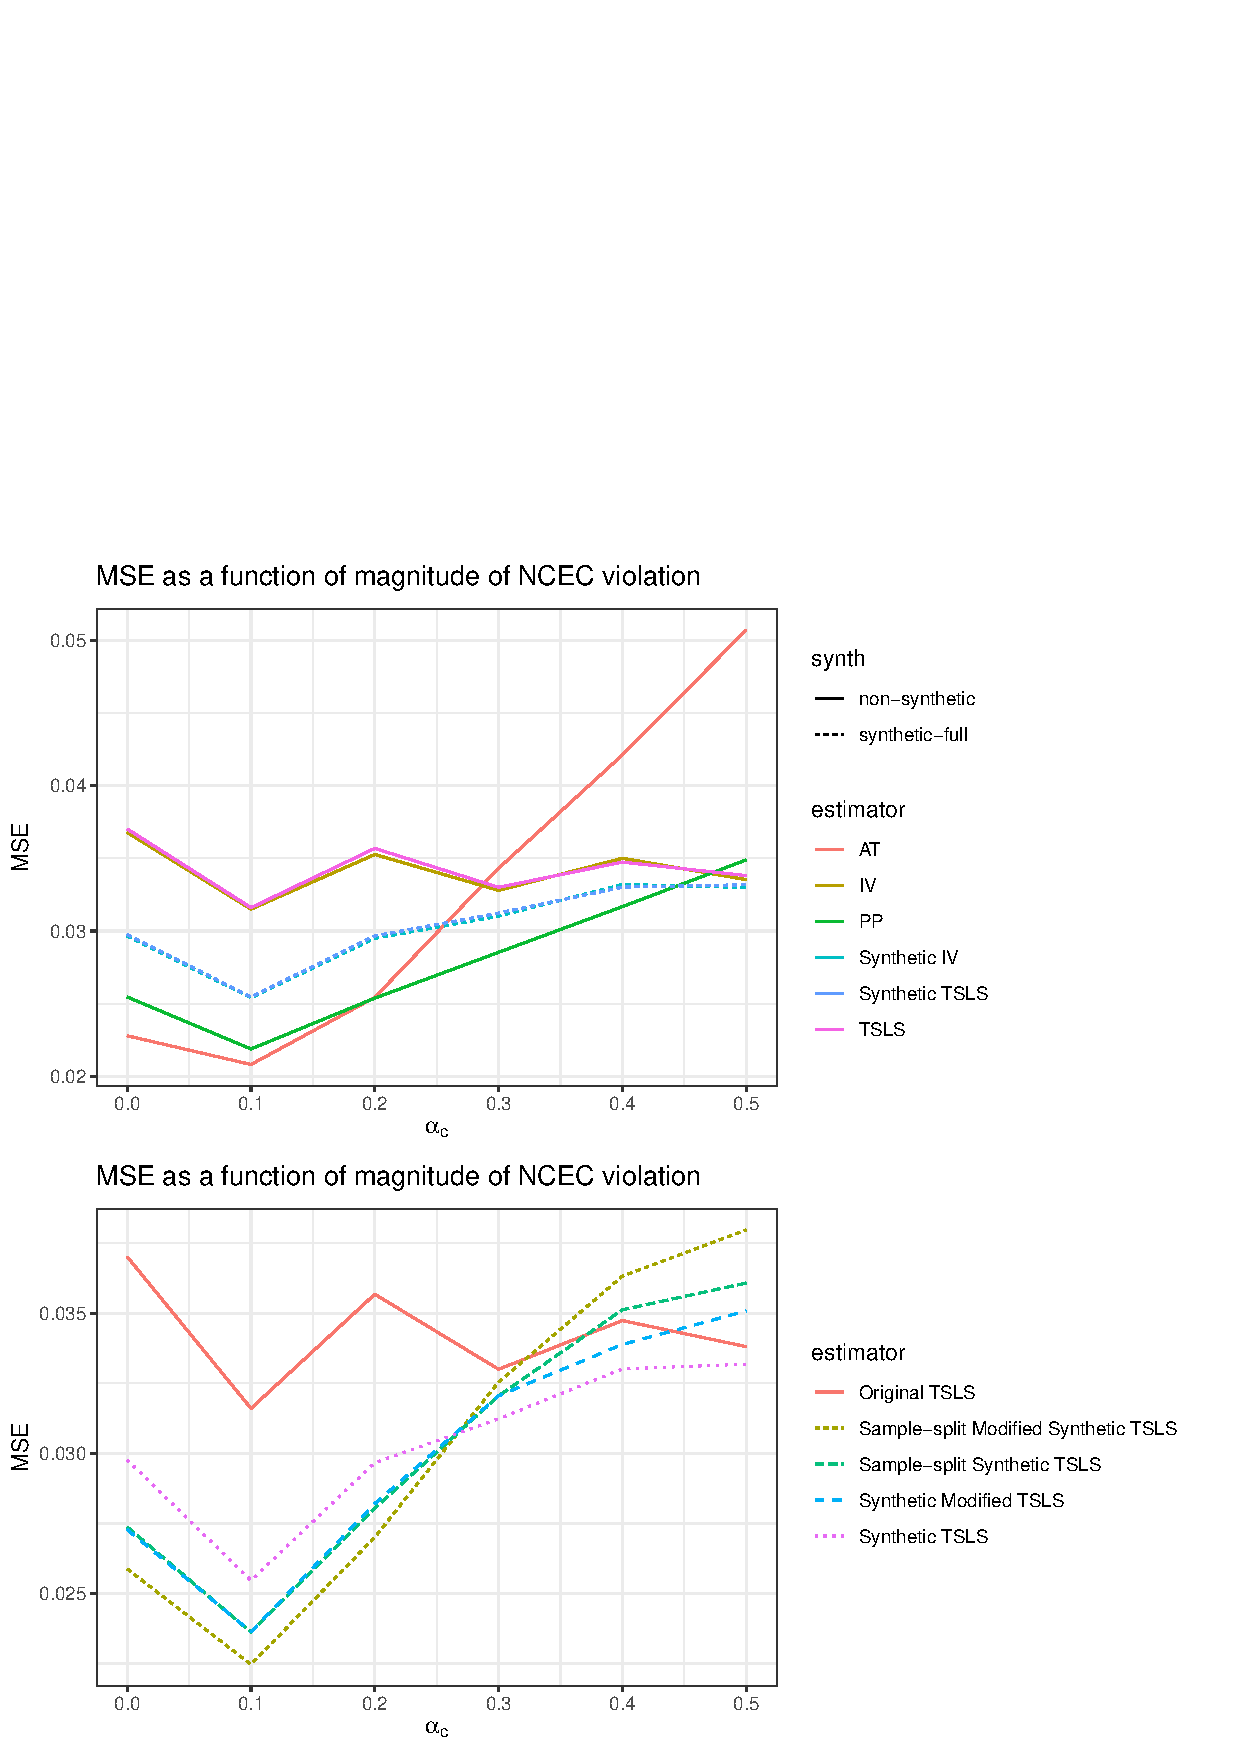
\includegraphics[width =\textwidth]{mse_bias_var_for_n200_cp06.pdf}
\end{tabular}\vspace{0.2in}
\caption{MSE, bias, and variance of the four candidate estimators and the two synthetic estimators as $\alpha_c$ changes. The sample size is $n = 200$, and the rest of the parameters are set to $\gamma_c = 0, \lambda_n = \lambda_c = 1, \beta_0 = 0.41, \beta_1 = 2$.}\label{mse_plot_1}
\end{figure}
%
The figure demonstrates that the synthetic estimator has a robustness property. When $\alpha_c$ is low the AT/PP estimators have the lowest MSE, but when $\alpha_c$ grows, the TSLS estimator begins to outperform them, while the IV estimator is always the worst because of its high variance. We see that theh Synthetic IV estimator always improves on the IV estimator in these settings by dramatically reducing its variance. The Synthetic TSLS estimator similarly improves on the TSLS estimator when AT/PP have low bias, but as they incur more and more bias, the performance of the Synthetic TSLS begins to mimic that of the TSLS estimator. 

\begin{figure}
\centering
\begin{tabular}{c}
%\includegraphics{figure_1_correlations.eps}
%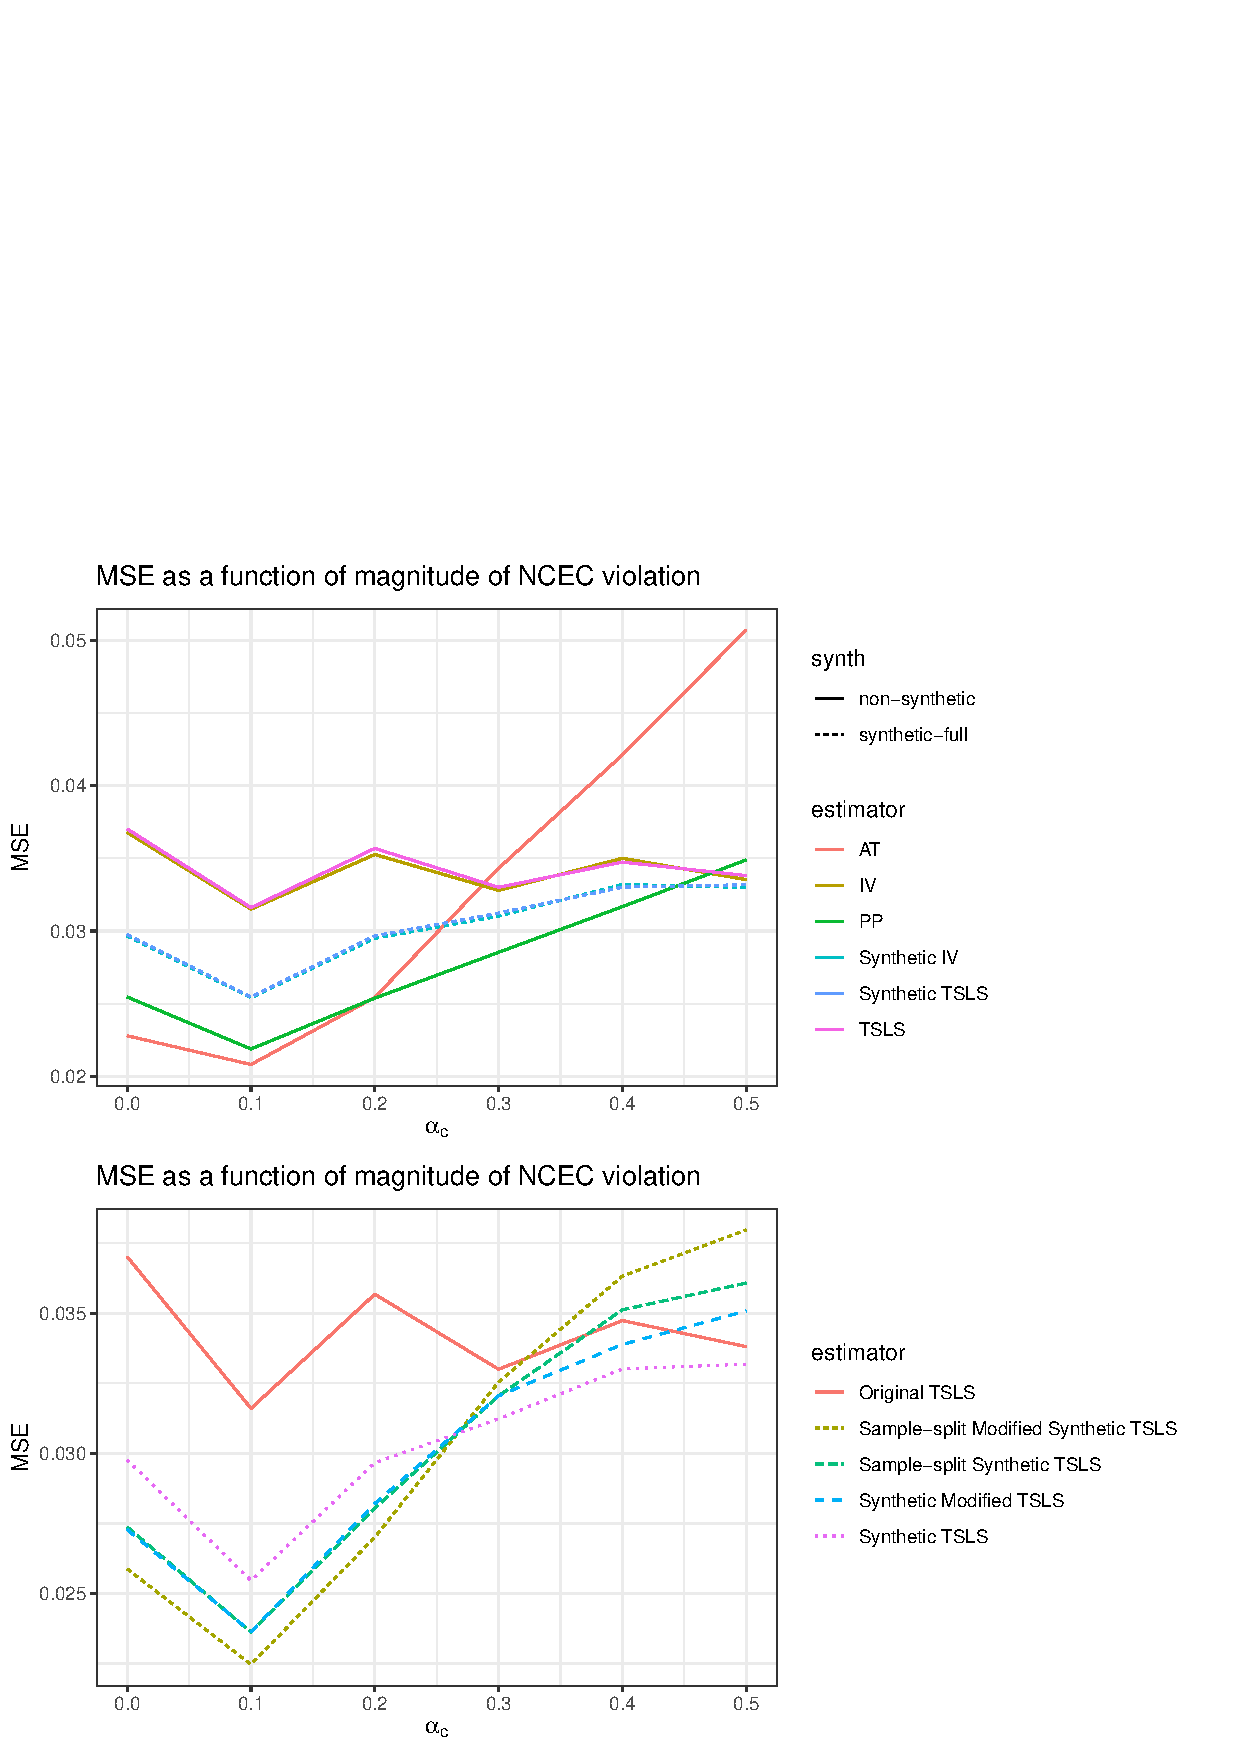
\includegraphics{mse_bias_var_for_n200_cp06.png}
\includegraphics[width =\textwidth]{mse_bias_var_for_n200_cp06_with_cv.pdf}
\end{tabular}\vspace{0.2in}
\caption{MSE, bias, and variance of the four candidate estimators and Synthetic TSLS and Sample-split Synthetic TSLS as $\alpha_c$ changes. The sample size is $n = 200$, and the rest of the parameters are set to $\gamma_c = 0, \lambda_n = \lambda_c = 1, \beta_0 = 0.41, \beta_1 = 2$.}\label{mse_plot_2}
\end{figure}
%
The performance of the sample-split synthetic estimator is demonstrated for the same settings in Figure \ref{mse_plot_2}. In the figure, the sample-split estimator unsurprisingly follows a similar trajectory to the Synthetic TSLS. The main difference is that the sample-split estimator is less tethered to the TSLS estimator: when the AT/PP estimators are best, the sample-split estimator benefits more than the Synthetic TSLS. On the other hand, when the AT/PP estimators are biased, the sample-split estimator is more sensitive to them and acquires a higher MSE compared to the SYnthetic TSLS.

\bibliography{compliance_refs}
\bibliographystyle{unsrtnat}

\end{document}

%\theta\right\}\sum_{j=1}^5\tdot_j(\bgamma_n)(\bgammahat_{nj} - \bgamma_{nj})\right],
%\] \\
%\end{split}\end{equation}
%\end{document}

